\documentclass[border=10pt]{standalone}
\usepackage[svgnames]{xcolor}
\usepackage{amsmath}
\usepackage{pgfplots}
\pgfplotsset{compat=newest}
\usepackage[sfdefault]{FiraSans}
\usepackage{FiraMono}
\renewcommand*\familydefault{\sfdefault}
\begin{document}
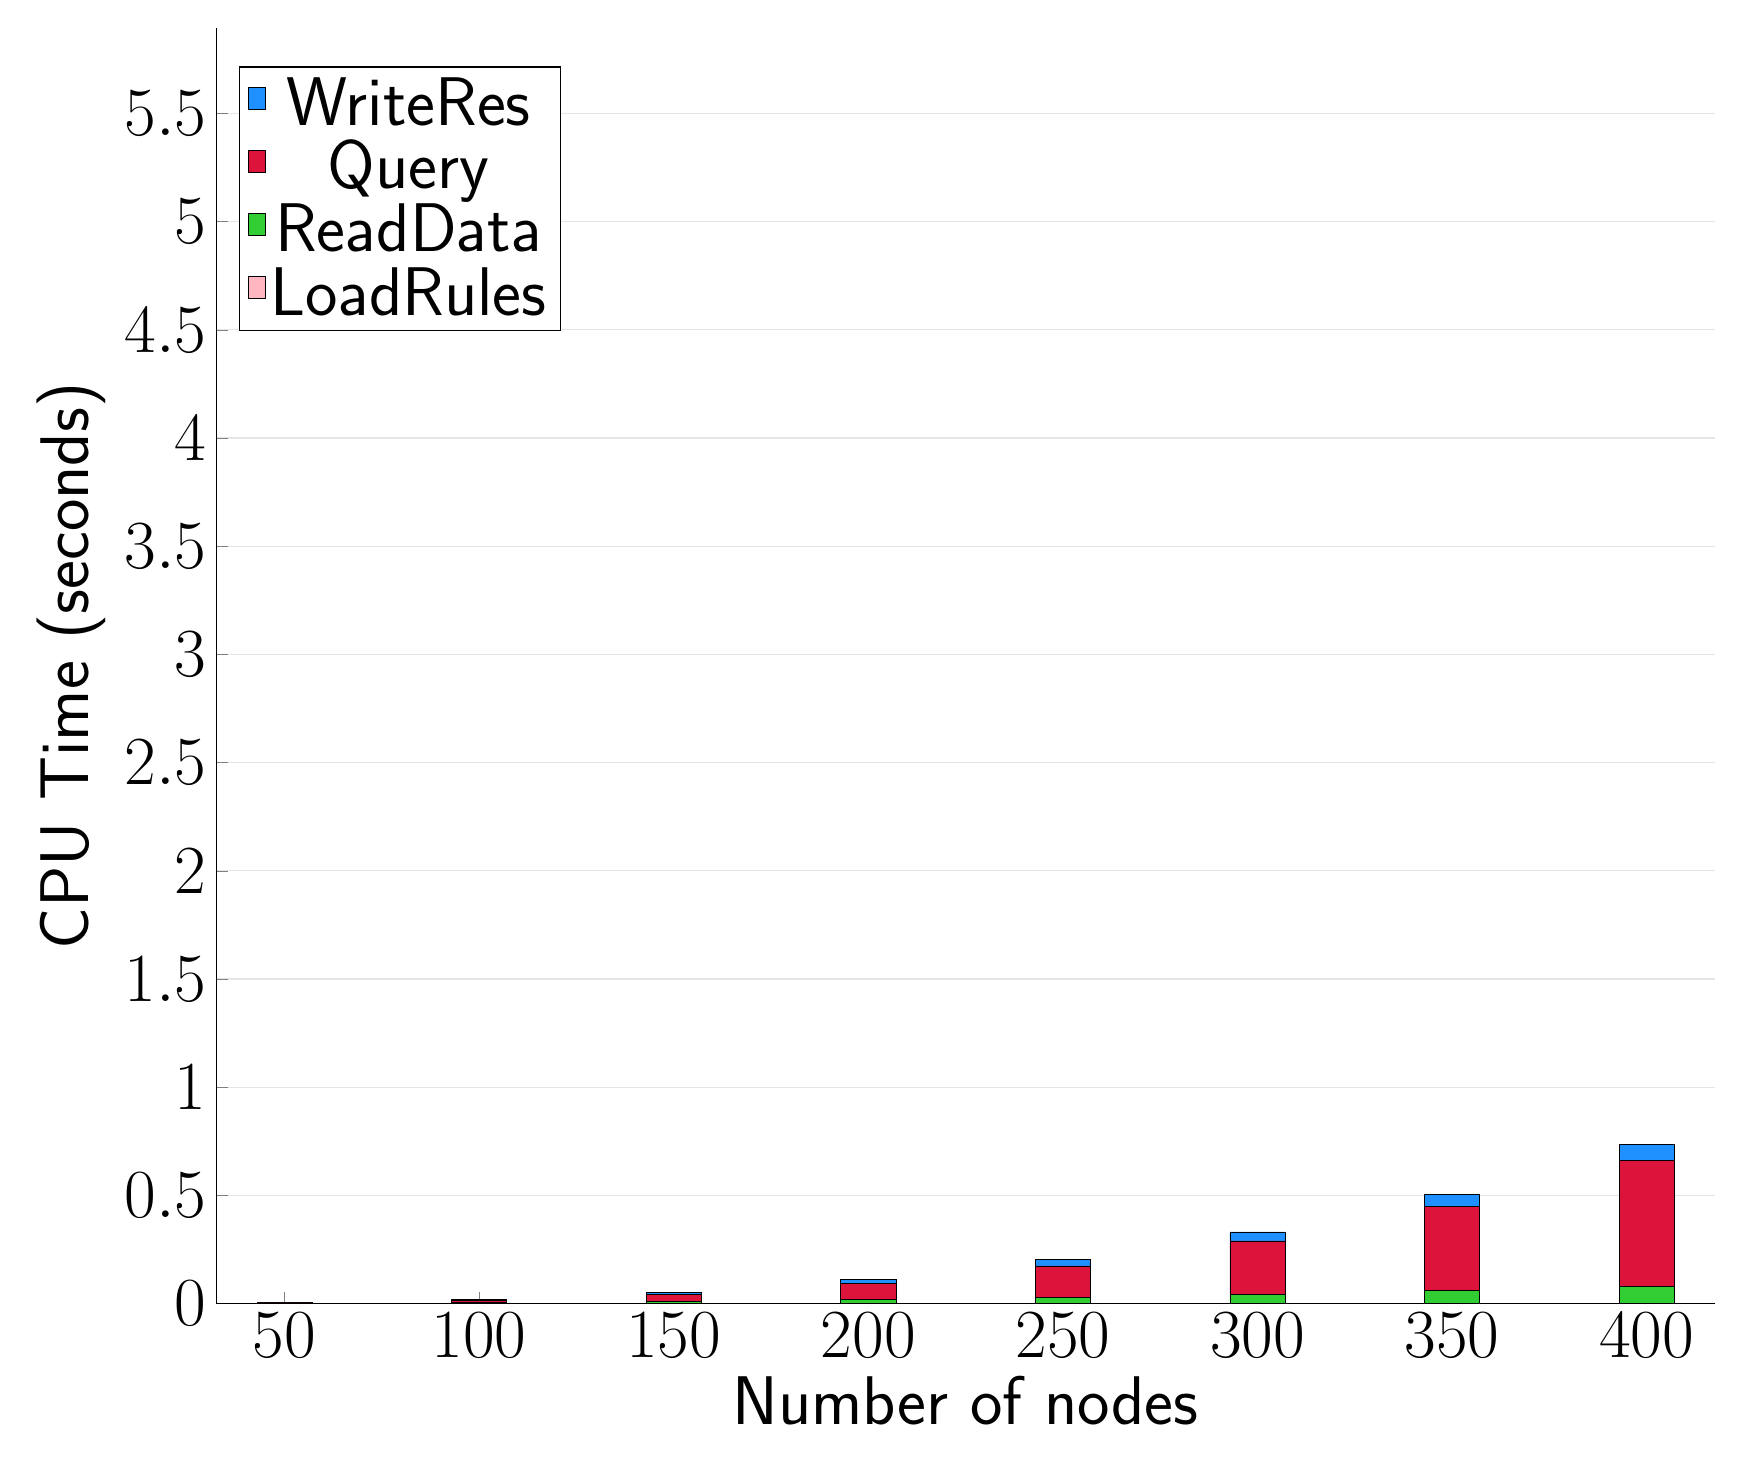
\begin{tikzpicture}
	\begin{axis}[
			ybar stacked,
			width=1.7\textwidth,
			bar width=0.7cm,
			ymajorgrids, tick align=inside,
			major grid style={draw=gray!20},
			xtick=data,
			ymin=0, ymax=5.893940000000001,
			axis x line*=bottom,
			axis y line*=left,
			enlarge x limits=0.05,
			legend style={
					at={(0.23, 0.97)},
					anchor=north east,
					legend columns=1,
					font=\Huge,
				},
			ylabel={CPU Time (seconds)},
			xlabel={Number of nodes},
			label style={font=\Huge},
			tick label style={font=\Huge},
		]
		\addlegendimage{fill=DodgerBlue, draw=black, line width=0.2pt}
		\addlegendentry{WriteRes}
		\addlegendimage{fill=Crimson, draw=black, line width=0.2pt}
		\addlegendentry{Query}
		\addlegendimage{fill=LimeGreen, draw=black, line width=0.2pt}
		\addlegendentry{ReadData}
		\addlegendimage{fill=LightPink, draw=black, line width=0.2pt}
		\addlegendentry{LoadRules}
		\addplot +[fill=LightPink, draw=black, line width=0.2pt] coordinates {
				(50, 0.0006271)
				(100, 0.0006166000000000004)
				(150, 0.0006108999999999996)
				(200, 0.0006007999999999996)
				(250, 0.0005962999999999998)
				(300, 0.0006098000000000001)
				(350, 0.0006278999999999996)
				(400, 0.0006121)
			};
		\addplot +[fill=LimeGreen, draw=black, line width=0.2pt] coordinates {
				(50, 0.0011819)
				(100, 0.0044548999999999995)
				(150, 0.0102316)
				(200, 0.0185252)
				(250, 0.029668099999999996)
				(300, 0.04331809999999999)
				(350, 0.060356900000000005)
				(400, 0.0799406)
			};
		\addplot +[fill=Crimson, draw=black, line width=0.2pt] coordinates {
				(50, 0.0012682000000000001)
				(100, 0.0094437)
				(150, 0.0312102)
				(200, 0.073782)
				(250, 0.1443604)
				(300, 0.24582600000000002)
				(350, 0.3891722)
				(400, 0.5827848)
			};
		\addplot +[fill=DodgerBlue, draw=black, line width=0.2pt] coordinates {
				(50, 0.0011434)
				(100, 0.004635599999999999)
				(150, 0.0104344)
				(200, 0.017969600000000002)
				(250, 0.029538999999999992)
				(300, 0.04214179999999999)
				(350, 0.0556636)
				(400, 0.07121339999999997)
			};
	\end{axis}
\end{tikzpicture}

\end{document}
